\chapter{Stellar rotation period inference using Gaussian processes}
\section{Introduction}

The light curves of spotted, rotating stars are often non-sinusoidal and
Quasi-Periodic (QP).
These stars vary in brightness due to active regions on their surfaces which
rotate in and out of view.
The non-sinusoidal quality is caused by the complicated surface spot patterns
and the quasi-periodicity is caused both by the finite lifetimes of these
active regions and the presence of differential rotation.
A strictly periodic sinusoid is therefore not a good representative
model for the light curves of FGK stars.
In an ideal world, a physical model of the stellar surface would be
conditioned on the data.
A physically realistic generative model would perfectly capture the
complexity of shapes within stellar light curves as well as the
quasi-periodic nature, allowing for extremely precise probabilistic period
recovery.
However, such physical models must have many free parameters in order to
accurately represent a stellar surface and these parameters are extremely
degenerate.
For example, as well as global stellar parameters such as inclination and
rotation period, each spot or active region should have (at minimum) a
longitude, latitude, size, temperature and lifetime.
Considering that many stars have on the order of hundreds of spots CITATION,
the number of free parameters quickly becomes unwieldy, especially if the
posterior PDFs of these parameters are explored with MCMC.
Simplified spot models, such as the one described in \citet{lanza}, where
only two spots are modelled, have produced successful results, however these
simplified models sacrifice some precision due to lack of model flexibility.
Instead of using a physical model for stellar light curves, we choose to use
an {\it effective} model.
One which captures the behaviour but is not physically motivated (although
the parameters of this model may be interpreted as physical ones).
An ideal effective model for the light curve of a spotted, rotating star is
one with a small number of non-degenerate parameters that is flexible enough
to perfectly capture non-sinusoidal, QP behaviour.
These requirements are perfectly fulfilled by a Gaussian process (GP) model.

The standard methods used for measuring rotation perids are detecting peaks in
a Lomb-Scargle (CITATION) (LS), sine-fitting periodograms
\citep[e.g.][]{reiners}, Auto-Correlation Functions (ACFs)
\citep{mcquillan2013} and wavelet transforms \citep{garcia2014}.
The efficacy of the LS periodogram and the wavelet methods are limited by the
suitability of the model choice.
In the case of the LS periodogram, the sinusoid is not an ideal model, as
described above, and the wavelet method similarly relies on a choice of mother
wavelet that should match the data over a range of transpositions.
The ACF method is much better suited to signals that are non-sinusoidal, in
fact it doesn't matter what shape the signal is---as long as it is periodic,
the ACF will contain peaks located at the period.
However, the ACF method requires data to be evenly-spaced, which is not the
case with \Kepler light curves (although in many cases it can be approximated
as uniformly sampled).
It is also an operation performed on the data, not a generative model of the
data and is therefore not probabilistic.
It is very difficult to estimate the uncertainty on a rotation period
measurement for this reason.
Many rotation periods in the literature have been inferred by measuring the
position in the first peak of an ACF, however this approach can be dangerous.
The exponential decay in correlation can shift the peak position to the left
of its true value, leading to an underestimate of the period.
In order to avoid this, a period should be inferred by modelling the entire
ACF, not just measuring the position of the first peak.

The motivation for developing a GP-based method for rotation period inference
is firstly, to measure more accurate and precise rotation periods using a
better-suited generative model than a sine-fitting periodogram for the
reasons explained above.
Secondly, to infer {\it probabilistic} periods, i.e. to estimate the
posterior PDF of the rotation period and thereby measure a realistic and
representative uncertainty.
Thirdly, to allow for an additional noise model to be included during
regression, the parameters of which could be marginalised over.
Fourthly to provide some way of determining whether a periodic model is
supported by the data over a purely stochastic one.

GPs are commonly used in the machine learning community and increasingly
in other scientific fields, for example biology and geophysics (where GP
regression is called `krigging').
They are useful in regression problems involving a stochastic process,
specifically when the probability distribution for the process is a
multi-variate Gaussian.
If the probability of obtaining a data set, generated by some process, is a
Gaussian in $N$ dimensions, where $N$ is the number of data points, that data
set can be described as and {\it with} a Gaussian process.
Gaussian process models parameterise the covariance between data points to
describe the data.
A kernel function provides the parameterisation of the covariance matrix.
For example, take the time-series in figure \ref{fig:GP_example}.
This is a \kepler\ light curve of Earth-like planet host Kepler-452, a G-type
star that rotates once every $\sim$ 15 days.
The variability visible in this time-series is typical of \kepler\ FGK stars.
It has been fit with a GP model, shown in orange.
Since GPs are flexible models, a range of kernel functions could be used to
describe the variability of Kepler-452.
For example, the simplest and most commonly used kernel function, the
'Squared Exponential' (SE) could produce an adequate fit to these data.
The SE kernel function is defined as,
\begin{equation}
k_{i,j} = A \exp \left(-\frac{(x_i - x_j)^2}{2l^2} \right).
\end{equation}
\label{eq:SE}
The SE kernel function has the advantage of being very simple---it has just
two parameters, $A$, the amplitude of covariance and $l$ the exponential
length scale of covariance decay.
If $l$ is large, two data points very far apart in $x$ will be tightly
correlated, and vice versa.
The SE kernel function may be an adequate model of the covariance in stellar
light curves, but it is not a `useful' one because it does not have a
parameter that controls a period.
In order to infer a rotation period, it is necessary to use a periodic kernel
function and to optimise the parameter that controls the period.
For this reason, we use the `Quasi-Periodic' (QP) kernel function for the
inference of stellar rotation periods.
The QP kernel function is defined as
\begin{equation}
k_{i,j} = A \exp \left(-\frac{(x_i - x_j)^2}{2l^2} -
\frac{\sin(\frac{2\pi}{P})^2}{\Gamma^2} \right).
\end{equation}
\label{eq:QP}
It is the product of the SE kernel function which describes the overall
covariance decay and an exponentiated, squared, sinusoidal kernel function,
that describes the periodic covariance structure.
$P$ can be interpreted as the rotation period of the star and $\Gamma$ is
related to the number of zero crossings per period.
$\Gamma$ may be related to the number of active regions on the stellar
surface, however investigating the connections of these hyper-parameters to
physical properties of the stars (other than rotation period) is beyond the
scope of this project.
This kernel function allows two data points that are separated in time by one
rotation period to be tightly correlated, while points separated by half a
period are weakly correlated.
This kernel function was used to produce the orange model shown in figure
~\ref{fig:GP_example}.
In order to infer a stellar rotation period from a light curve, a GP model
with a QP covariance function is fit to the data.
The likelihood of the model, conditioned on the data could then be maximised
in order to find the maximum likelihood value for $P$.
Alternatively, and as we do in this study, the posterior PDFs of the
hyper-parameters are explored using MCMC.
This latter approach comes at a cost: a GP model is expensive to compute
once, let alone however many thousands of times is necessary to fully explore
the posteriors of the parameters.
However, it fully maps out the posterior PDF of $P$, which is one of the
primary goals of this alternative approach to rotation period inference.

\begin{figure}
\begin{center}
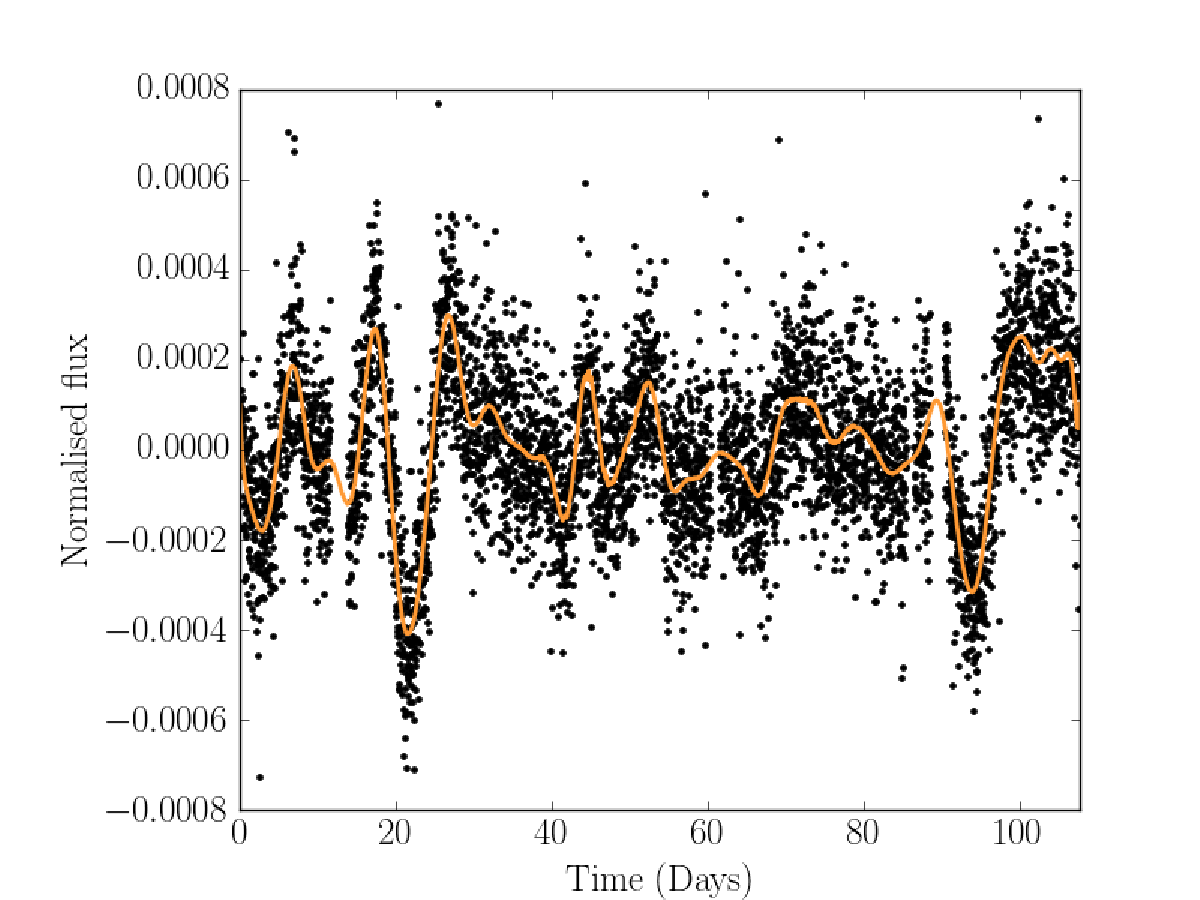
\includegraphics[width=6in, clip=true]{figures/Kepler452b.pdf}
\caption{Light curve of Kepler-452 b, a habitable-zone, Earth-sized planet
hosting G star \citep{jenkins}. The orange line shows a fit to the data using
a Gaussian process model with a QP covariance kernel function.}
\label{fig:GP_example}
\end{center}
\end{figure}

\section{Application}

In order to infer a rotation period from a light curve, we attempted to
measure rotation periods of three sets of light curves: simulated noise-free,
simulated noisy and real light curves.

\section{Rotation period recovery (noise-free)}

\subsection{ACF}

We calculated an ACF for each light curve using the method of
\citet{mcquillan13}.
In this method, an ACF is calculated and smoothed with a Gaussian kernel for
each light curve.
A rotation period is estimated as the lag-time of the first peak in the ACF,
unless the second peak is larger in which case {\it that} lag-time is
interpreted as the true period.
The second peak in an ACF can be larger than the first if there are two active
regions at or near opposite longitudes on the surface of the star---this would
produce a light curve with two dips per rotation period.
By extension, if three active longitudes existed at 60$^\circ$ separations on
the stellar surface, one third of the true rotation period would be measured,
and so on.
An example ACF of the light curve in figure~\ref{fig:noise-free_lc} is shown
in figure~\ref{fig:ACF_example}.

\begin{figure*}
\begin{center}
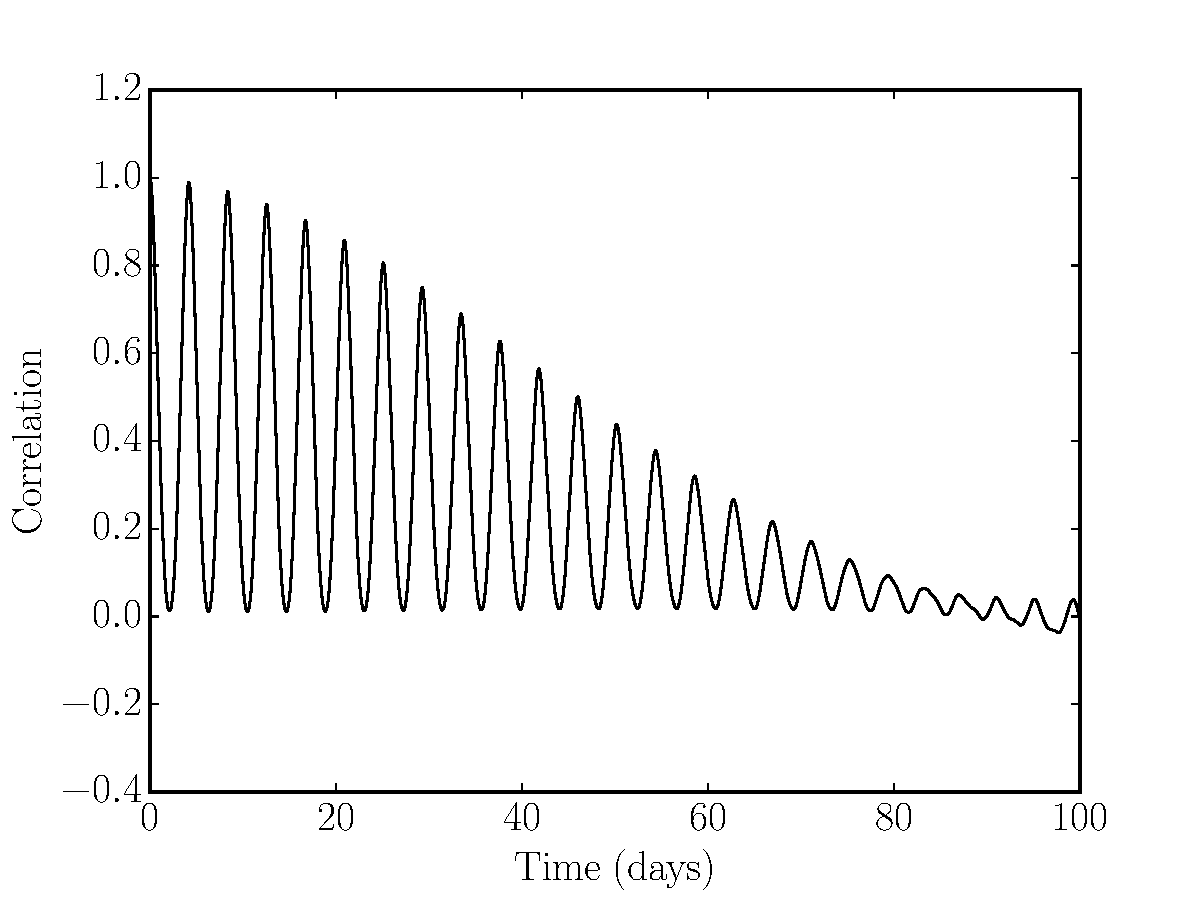
\includegraphics[width=6in, clip=true]{figures/noise-free_acf.pdf}
\caption{The autocorrelation function of the simulated, noise-free light
curves depicted in figure \ref{fig:noise-free_lc}.}
\end{center}
\end{figure*}
\label{fig:compare_noise_free}

This method has proven to be extremely useful for measuring rotation periods.
The catalogue of rotation periods of \Kepler stars provided in
\citet{mcquillan2013} has been widely used by the community and has provided
ground-breaking results for stellar and exoplanetary science.
The results of the ACF method as tested in \citet{aigrain2015} were
encouraging (see, for example their figure 8) as it produced a large number of
accurate rotation period measurements.
The ACF method is also conveniently fast to implement.
The periods measured using the ACF method are plotted against the `true'
rotation period values used to generate the simulated noise-free light curves
in figure \ref{fig:acf_compare_noise-free}.
73\% of the injected rotation periods were recovered with a value lying
within 10\% of the truth and 83\% within 20\%.
A noteworthy feature of this figure is that many of the points fall below the
$x=x$ line, \ie the recovered rotation periods are a little shorter than the
true periods.
We believe this is caused by the peak position measurement performed on the
ACF.
ACFs of stellar light curves can be roughly described as a cosine function
superimposed on top of a decaying exponential.
In such a function the peak positions can be shifted towards the 'left', \ie
the short period end, because the decaying exponential raises the left side of
each peak more than the right.
It is possible to model this effect, of course, however the standard practise
is to simply measure the peak position without taking this effect into
account.
To demonstrate that this effect reproduces the underestimated periods seen in
figure \ref{fig:compare_noise-free}, we generated 1000 ACFs by adding cosine
and exponential functions with a range of periods, decay timescales and
relative amplitudes.
The measured position of the first peak was compared to the true position as
demonstrated in figure \ref{fig:exp_sine_test}.
The same underestimation of the peak position is demonstrated in this figure.

\begin{figure*}
\begin{center}
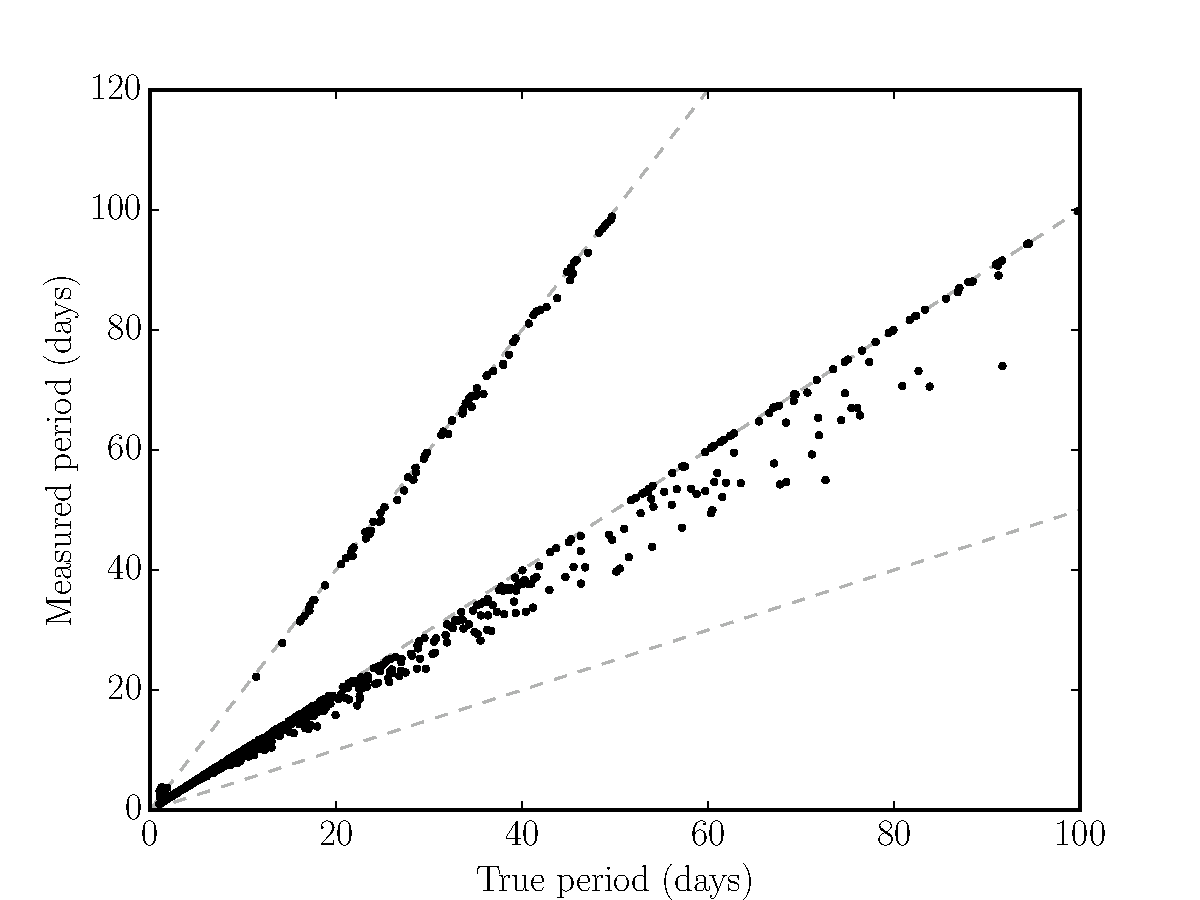
\includegraphics[width=6in, clip=true]{figures/exp_sine_test.pdf}
\caption{Recovered peak position as a function of the `true' period used to
generate simulated ACFs. In many cases the position is measured short-wards of
the truth as also seen in figure \ref{fig:compare_noise_free}.}
\end{center}
\end{figure*}
\label{fig:exp_sine_test}

\begin{figure*}
\begin{center}
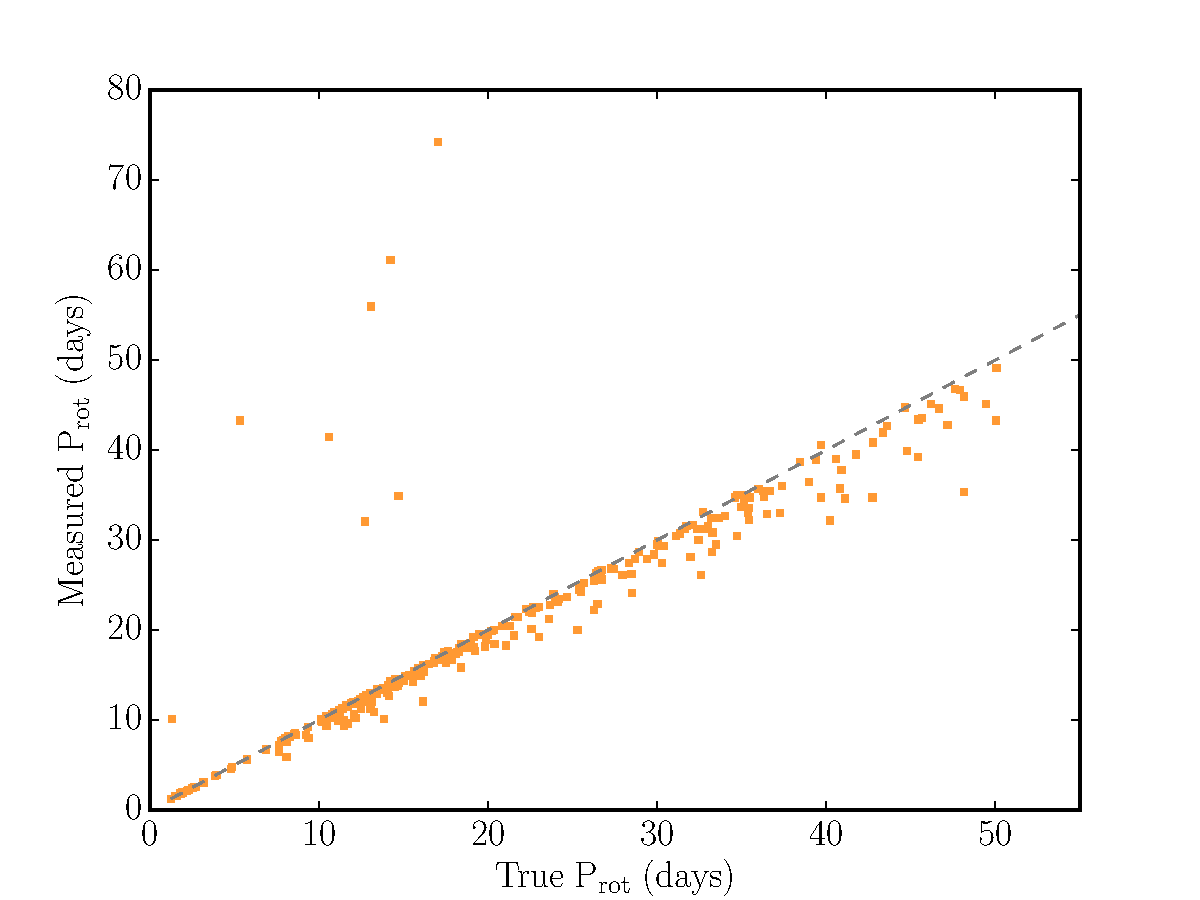
\includegraphics[width=6in, clip=true]{figures/acf_compare_noise-free.pdf}
\caption{Recovered rotation periods as a function of the `true' rotation
period used to generate 330 simulated light curves.}
\end{center}
\end{figure*}
\label{fig:compare_noise_free}

\subsection{The sine-fitting periodogram method}

For each simulated, noise-free light curve, a LS periodogram was computed for
10,000 periods (spaced evenly in frequency) between 1 and 100 days.
The period of the highest peak in the periodogram was adopted as the period.
The resulting recovered rotation periods plotted as a function of the true
periods are shown in figure \ref{fig:pgram_compare_noise-free}.
These recovered rotation periods are, in general more accurate than the ACF
results, they do not systematically over or under predict rotation period.
The unsuccessful recoveries which happen preferentially for the shorter
rotation periods are caused by fluctuations in the light curve produced by
changes in the total spot coverage on the stellar surface.
These fluctuations can be larger in magnitude than those produced by the
rotational signal itself.

\begin{figure*}
\begin{center}
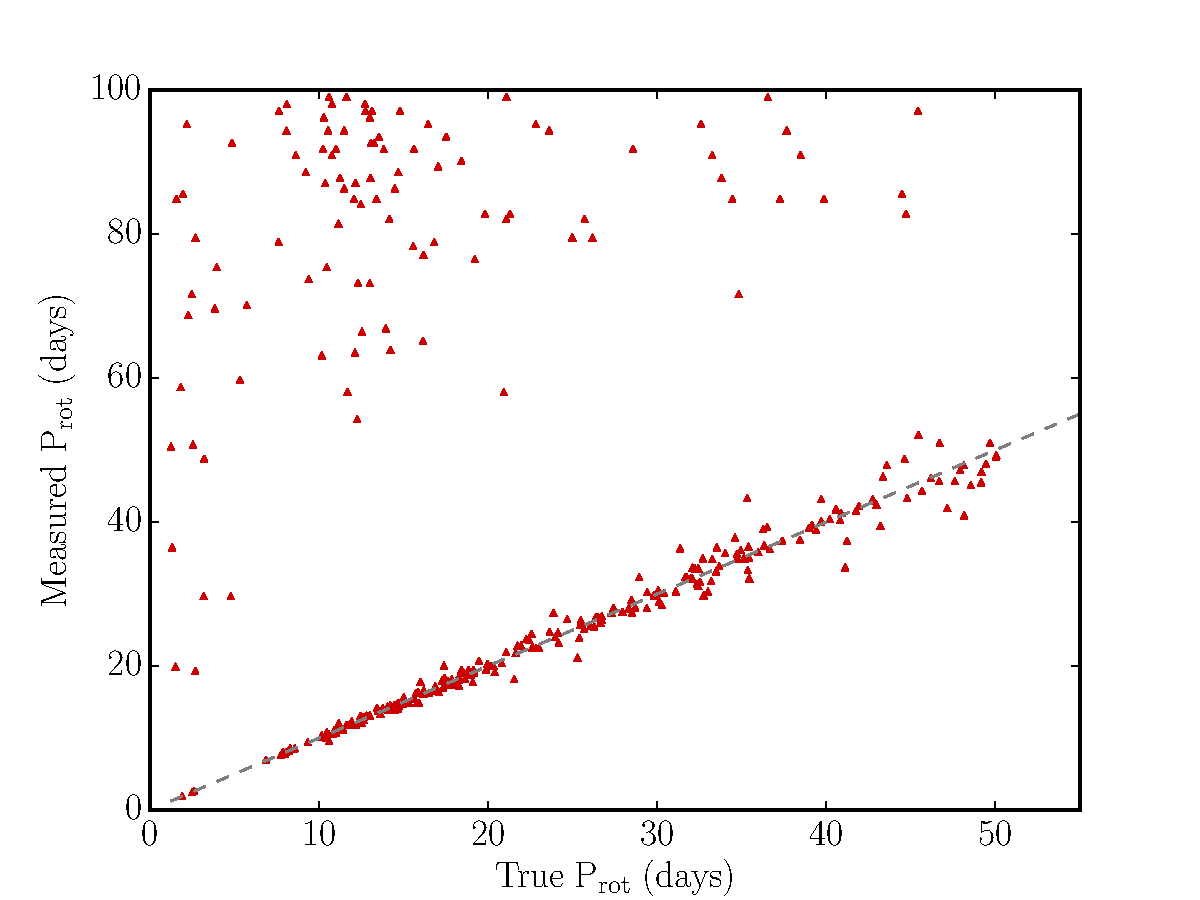
\includegraphics[width=6in, clip=true]{figures/pgram_compare_noise-free.pdf}
\caption{Recovered rotation periods as a function of the `true' rotation
period used to generate 330 simulated light curves.}
\end{center}
\end{figure*}
\label{fig:compare_noise_free}

\subsection{The GP method}

In order to recover the rotation periods of the simulated light curves using
Gaussian processes we sampled the posterior PDFs of the kernel hyperparameters
described in equation \ref{eq:QP}.
The likelihood function for a GP is similar to the simple Gaussian likelihood
function that is used for optimisation problems where the uncertainties are
Gaussian and uncorrelated, the logarithm of which is also known as
$-\frac{1}{2}\chi^2$.
This likelihood function can be written
\begin{equation}
\ln \mathcal{L} = -\frac{1}{2}\sum_{n=1}^N\frac{(y_n-\mu)^2}{\sigma_n^2}
    - \frac{N}{2}\ln(2\pi\sigma_n^2),
\end{equation}
\label{eq:chi2}
where $y_n$ are the data, $\mu$ is the mean model and $\sigma_n$ are the
Gaussian uncertainites on the data.
The equivalent equation in matrix notation is
\begin{equation}
\ln \mathcal{L} = -\frac{1}{2}\bf{r}^T\bf{C}^{-1}\bf{r}-\ln|\bf{C}|
    + \mathrm{constant},
\end{equation}
\label{eq:lhf1}
where $\bf{r}$ is the vector of residuals and $\bf{C}$ is the covariance
matrix,
\begin{eqnarray}
	\mathbf{A} &=& \left (\begin{array}{cccc}
	\sigma^2_1 & \sigma_{2, 1} & \cdots & \sigma_{N, 1} \\
	\sigma_{1, 2} & \sigma^2_2 & \cdots & \sigma_{N, 2} \\
    && \vdots & \\
	\sigma_{1, N} & \sigma_{2, N} & \cdots & \sigma^2_N
\end{array}\right )
\end{eqnarray}
In the case where the uncertainties are uncorrelated, the noise is `white',
(which is a frequent assumption made by astronomers and is sometimes
justified) the off diagonal elements of the covariance matrix are zero.
However, in the case where there is justifiable evidence for correlated noise,
as in the case of \Kepler light curve modelling, those off-diagonal elements
are non-zero and are, in fact, exactly what we are trying to model.
In the GP case, a covariance matrix generated by the kernel function, ${\bf
K}$ replaces ${\bf C}$ in the above equation.
Incidentally, this approach is the reverse of the regression techniques
usually employed by astronomers.
In most problems in astronomy you try to understand the parameters that
describe your mean model and, if correlated noise is present, to marginalise
over that noise.
Here, the {\it noise} is what we are interested in and our mean model is
simply a straight line at $y=0$.

One could either maximise this likelihood function in order to find the
best-fit hyperparameters of the covariance kernel function or, as in our
approach, sample from the posterior PDFs of the hyper-parameters.
The advantage of the maximum-likelihood method is that the best-fit parameters
will be found much faster, however the uncertainities on the rotation period
will not be constrained.
In order to measure accurate uncertainties the posterior PDFs of the
parameters must be explored.
Since obtaining accurate uncertainties on rotation periods is one of our main
motivations for this method, we use MCMC despite the added computational
expense.

We use the ACF period as an initial guess for the rotation period (this
decision is discussed further in section \textsection{section:discussion}).
We use uniform prior over rotation period with bounds described below and
assert that the covariance decay timescale parameter, $l$ must be greater than
the rotation period.
This represents our assumption that active regions have greater
For the remaining hyperparameters we use the following initial values and
log-uniform prior distributions:
\begin{eqnarray}
 	&	A_{initial} = e^{-5}, \sim U(\exp[-20:20]) \\ \nonumber
 	&	l_{initial} = e^{7}, \sim U[\exp(-20:20)], l<P \\ \nonumber
 	&	\Gamma_{initial} = e^{0.6}, \sim U([\exp(-20:20)]) \\ \nonumber
 	&	\sigma_{initial} = e^{-16}, \sim U([\exp(-20:20)]) \\ \nonumber
 	&	P_{initial} = P_{ACF}, \sim U((1 - 0.4)P_ACF < P_ACF < (1 + 0.4)P_ACF).
 \end{eqnarray}
 \label{eq:initialisation}

% The GP likelihood function howe Using the ACF period as
% an initial guess, we then subsample the light curves and split them into
% \kepler quarters in order to reduce computation time.
% The subsampling reduces computation time simply by contracting the data
% set---the HODLR solver scales as $N \log ^2 (N)$.

\begin{figure*}
\begin{center}
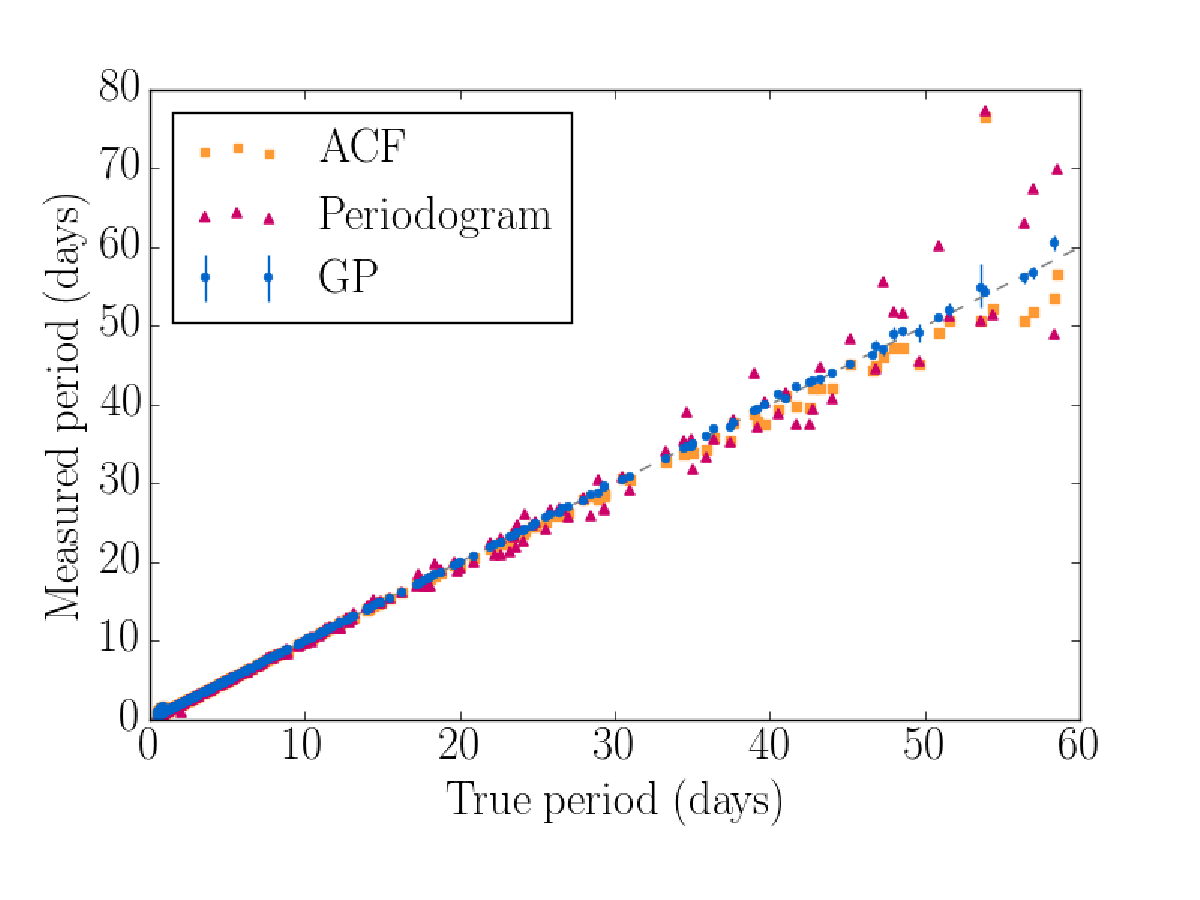
\includegraphics[width=6in, clip=true]{figures/compare2.pdf}
\caption{Measured vs true rotation period for 300 simulated light curves.}
\end{center}
\end{figure*}
\label{fig:compare_noise_free}

\section{Rotation period recovery (with noise)}

We used light curves simulated for the \citet{aigrain15} `hare and hounds'
rotation period recovery experiment.
The light curves were simulated by placing dark, circular spots, whose size
slowly evolves, on the surface of rotating stars.
\citep{aigrain15} simulated one thousand light curves in order to test the
ability of participating teams to recover both the stellar rotation periods
and the rotational shear: the amplitude of surface differential rotation.
We are not interested in recovering differential rotation and so only use
light curves simulated {\it without} differential rotation, of which there are
330.
We opt to use the solid-body rotators because differential rotation may
produce some additional scatter in the rotation period measurements we recover
that has a physical origin, rather than being the result of a flawed method.
The ranges and distributions of the physical stellar parameters used in the
simulated light curves are tabulated below in table
\ref{tab:simulation_parameters}.

\begin{table*}
\begin{center}
\caption{Ranges and distributions of parameters used to simulate light curves
in \citet{aigrain15}}
\begin{tabular}{lcc}
\hline\hline
    Parameter & Range & Distribution \\
    \hline
    Rotation period, $P_{rot}$ & 10 - 50 days (90\%) & log uniform \\
    & 1 - 10 days (10\%) & log uniform \\
    Activity cycle length & 1 - 10 years & log uniform \\
    Inclination & 0 - 90$^\circ$ & Uniform in $\sin^2i$ \\
    Decay timescale & (1 - 10) $\times P_{rot}$ & log uniform \\
\hline
\end{tabular}
\end{center}
\end{table*}
\label{tab:simulation_parameters}

Ideally, simulated light curves would be injected into the pixel-level data,
then the same detrending method that is applied to the \kepler light curves
would be applied to these simulations before attempting to measure rotation
periods for these stars.
However, since this work is designed to be more of a demonstration of the
efficacy of the GP periodogram, rather than the development of a \Kepler data
specific method, this is beyond the scope of our demonstrations.
\begin{figure}
\begin{center}
% 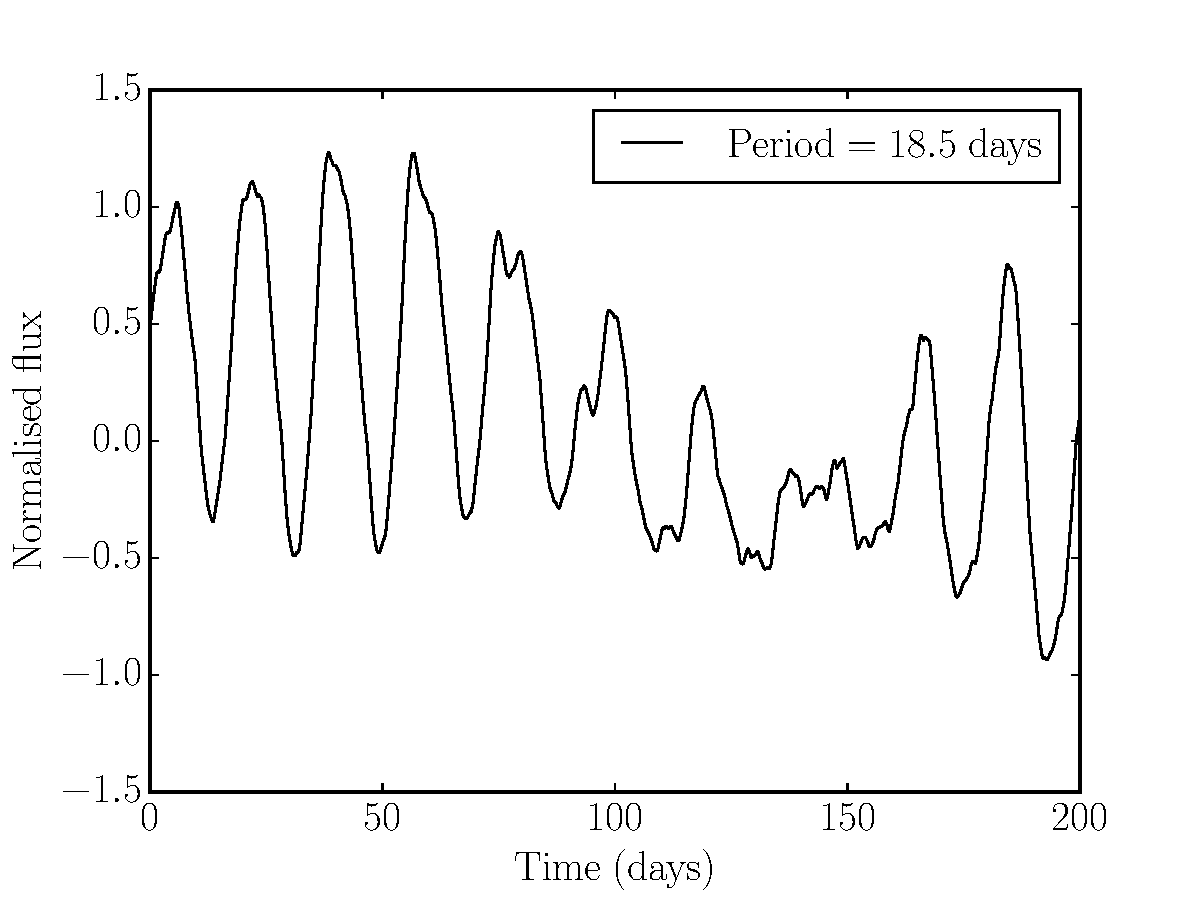
\includegraphics[width=6in, clip=true]{figures/noise-free_lc.pdf}
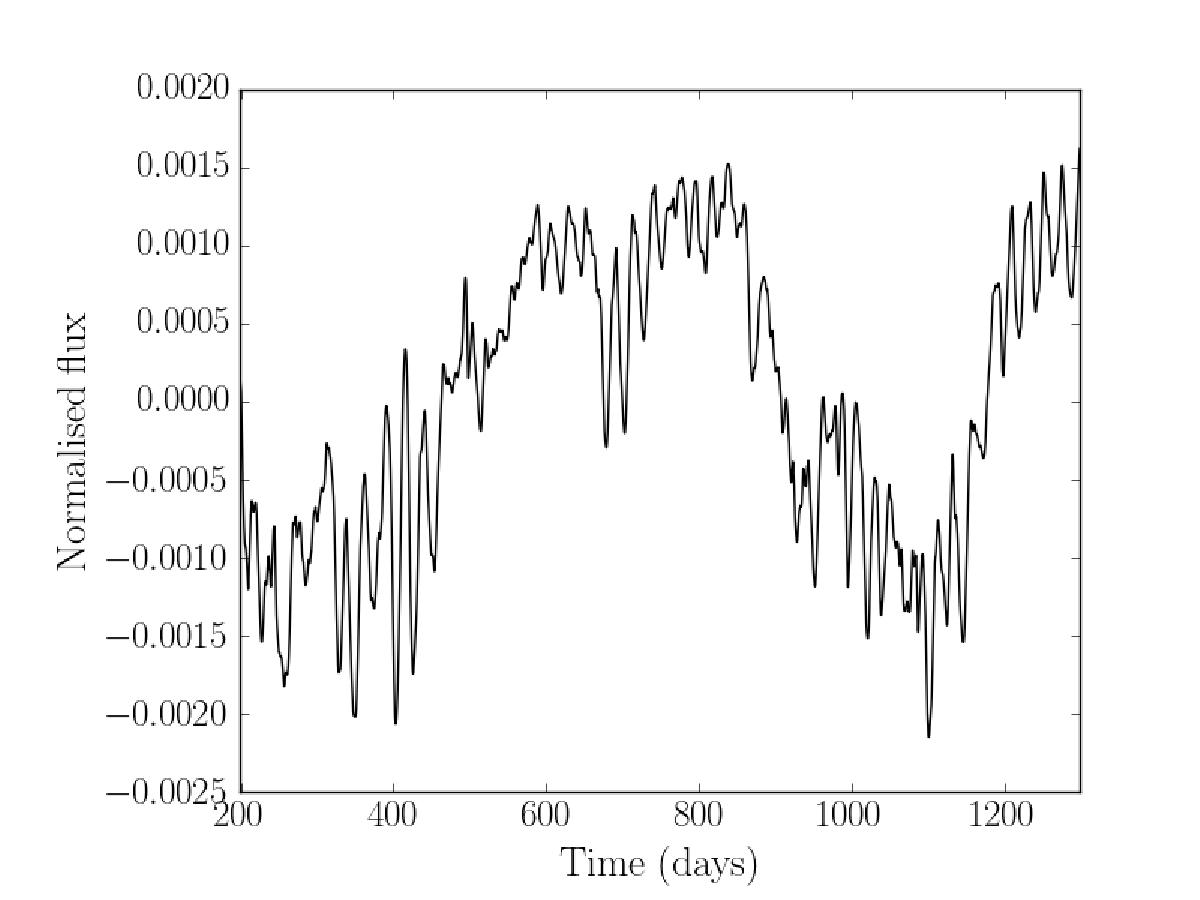
\includegraphics[width=6in, clip=true]{figures/thesis_plot.pdf}
\caption{An example simulated, noise-free light curve. This `star' has a
rotation period of 17.4 days.}
\label{fig:noise-free_lc}
\end{center}
\end{figure}
Figure \ref{fig:noise-free_lc} shows an example of a simulated light curve
with a period of 17.4 days.

We attempted to recover the rotation periods of these 330 light curves, both
with and without noise, (\ie before {\it and} after being injected into
\kepler light curves) using three rotation period recovery methods: the ACF
method, the sine-fitting periodogram method and the GP method.

\subsection{\kepler data}
\kepler data provides an interesting practical problem.
The same unique precision and short integration times that make \kepler
data such an unprecedented scientific gold mine also renders it extremely
difficult to work with.
\kepler data is big data and extracting the maximum amount of information
from it requires either large numbers of CPU hours, or using work-arounds.
One feature of the \kepler data that works in our favour is that it is
naturally broken up into smaller time units by quarterly breaks.
Splitting the data set into quarters, rather than modelling the entire time
series contiguously speeds up the computation time as inverting several
small matrices is faster than inverting one large one.
The \kepler quarter divisions are natural places to split the time series
because the spacecraft rotates by ninety degrees every quarter (three months),
placing each star on a new CCD module.
Pixel response functions and background flux differs from pixel-to-pixel and
module-to-module, so noise properties of \kepler light curves change every
quarter.
Additionally, changes in the spacecraft's orientation and position during
quarterly re-pointings temporarily affect the temperature of the CCD,
producing systematic features in the light curves at the start of some
quarters.
We model each quarter separately, however the parameters of the GP kernel
function are global, {\it i.e.} we do not use a separate period parameter for
each quarter---there is just one period parameter for an entire light curve.
It would be possible to model the time series with a mixture of some global
parameters and some quarter-specific parameters, for example one might expect
that the amplitude of covariance, $A$ or white noise level, $\sigma$ to vary
on a quarterly basis.
However, since there are seventeen quarters this would lead to thirty-seven
parameters, and in the interest of minimising computation time (adding
parameters leads to longer MCMC burn in and convergence time), we choose to
use global parameters only.

\section{Discussion}
\label{section:discussion}

\subsection{The ACF method}
The main advantage of the ACF method over the GP method is speed: it is
extremely fast and therefore useful to get a quick estimate of a period.
We have demonstrated that the ACF method may produce rotation periods that are
slightly systematically biased towards lower rotation periods.
This effect comes from the process of extracting the period from the ACF
itself: typically superimposed onto a decaying exponential, that first peak in
the ACF gets shifted towards faster periods.
One may be able to get around this by modelling the ACF as a sum of a cosine
and exponential function (a similar function to GP kernel function), however
in practise ACFs tend to have a more complicated structure and it is not
possible to model them with a simple function.
This observation leads to the idea of modelling the ACF with a Gaussian
processes, which then logically progresses to a using a Gaussian process with
a Gaussian process kernel function.
Although this may be an attractive (if somewhat mad) idea, in practise a GP
would not necessarily produce a positive semi-definite covariance
kernel\footnote{One that can be inverted; a necessary regression operation.}.
An alternative approach may be to correct for rotation period bias after the
peak position has been measured by inferring a correction factor.

\subsection{Initialisation}
Using the ACF to initialise the MCMC chains is not ideal because, of course,
you become reliant on the assumption that the ACF period is close to the true
period.
Of course, if you had infinite CPU time, this would not be a problem as you
would eventually sample the entire posterior PDF of the period parameter
however in practise this is likely to be an issue.
The only way to get around this problem is to run the MCMC chains for as long
as possible, or, alternatively to use a sampler that is designed to move
around the parameter space much more quickly than {\tt emcee}, for example
nested sampling.
We chose to use the ACF periods rather than the periodogram periods to
initialise as, although there was some systematic bias present in these
results, that bias was small and there were fewer large outliers.

\subsection{Kernel function choice and interpretation of hyper-parameters}
We are using a somewhat arbitrary mathematical function to describe a
physical process.
Another valid choice would be a cosine function multiplied by a squared
exponential,
\begin{equation}
k_{i,j} = A \exp \left(-\frac{(x_i - x_j)^2}{2l^2}\right)
\cos\left(\frac{2\pi}{P})^2{\Gamma^2}\right)
\end{equation}
\label{eq:cos_kernel}
This function produces a positive semi-definite matrix and has the $P$
parameter of interest.
This function may in fact be even {\it more} suited to modelling stellar
light curves as it describes a Gaussian in frequency space.
It is easy to imagine a differentially rotating star with a period that is a
Gaussian in frequency space: the mean frequency would be the frequency at the
most active latitude, at or near which spots spend the majority of their time
and the tails would be occupied by spots that drift near the equator or poles.
The main difference between this cosine and the QP function is that the cosine
function allows negative covariances and the QP function does not.
Is is realistic to allow negative covariances?
In practise, the ACFs of \Kepler light curves often go negative.
However, many stars have two active regions on opposite hemispheres that
produce two brightness dips per rotation.
If the covariance is forced to be negative for two data points that are
separated by half a rotation period, those light curves with two peaks per
rotation period may not be well modelled.
It would be very worthwhile to test this assumption and this alternative
kernel function in future.

Clearly, stellar rotation periods are well represented by the $P$ parameter in
our QP kernel function, as evidenced by the its impressive ability to recover
the true rotation periods from the simulated light curves in this work.
However, it is not clear whether the QP kernel function is the {\it best}
function to use.
There may be an alternative function which is better suited to capturing
stellar variability and is able to recover periods even more precisely than
the QP kernel.
There may also be an alternative function which is more physically motivated,
that captures not just the rotation period but also (for example) the spot
lifetime or differential surface rotation.
This is beyond the scope of this work but we hope that these questions will be
answered in the near future.
